\documentclass{subfiles}

\begin{document}


    \begin{Frage}
        Licht- Materie Wechselwirkung (Absorbtion und Emission).
    \end{Frage}
    \begin{Antwort}
        Es gibt hier im Groben drei interessante Fälle. Betrachte zunächst das Schaubild:
        \begin{figure}[H]
            \centering
            \includegraphics[width=8cm]{Bilddateien/AbsorptionEmission.png}
            \caption{Schematische Darstellung der Absorbtion und Emission von Licht durch ein Atom \cite{exp8-paper}.}
            \label{fig:AbsorptionEmission}
        \end{figure}
        \begin{enumerate}
            \item Die \emph{Absorbtion} von Licht durch ein Atom. Es liegt eine Proportionalität $\dv{t}N(t)\propto n_1\cdot u_{ph}$ vor, wobei $u_{ph}$ die Photonenenergiedichte ist. Der Proportionalitätsfaktor ist die \emph{Absorbtionsrate} $B_{1\to 2}$ (Einstein Koeffizient).
            \item Die \emph{induzierte Emission} von Licht durch ein Atom. Es liegt eine Proportionalität $\dv{t}N(t)\propto n_2\cdot u_{ph}$ vor, wobei der Proportionalitätsfaktor hier die \emph{induzierte Emissionsrate} $B_{2\to 1}$ ist.
            \item Die \emph{spontane Emission} von Licht durch ein Atom. Es herrscht hier eine Proportionalität $\dv{t}N(t) \propto n_2\cdot V$. 
        \end{enumerate}
        Man kann hier zeigen, daß $B_{1\to 2} = B_{2\to 1}$ gilt. 
        \begin{figure}[H]
            \centering
            \begin{subfigure}[t]{0.4\textwidth}
                \centering
                \includegraphics[width=\textwidth]{Bilddateien/StimulatedEmission.png}
                \caption{Induzierte Emission.}
                \label{fig:StimulatedEmission}
            \end{subfigure}
        \end{figure}
        Über die spontane Emission kann weiter eine \emph{Lebensdauer} $\tau$ definiert werden, welche die Lösung der vorgestellten Differentialgleichung der Form 
        \[
            n_2(t) = n_2(0)\cdot \exp(-A_{2\to 1}\cdot t)
        \]
        mit $\tau = 1/A_{2\to 1}$ ist. \\

        Die \emph{spektrale Linienbreite}, also der Energiewert, bei welchem spontane Absorbtion stattfindet, ist gegeben durch $\Delta E\cdot\delta t \geq \hbar/2$. Die Absorbtionslinie ist also nicht scharf, sondern folgt einer Gaußkurve mit Breite $\Delta E$:
        \begin{figure}[H]
            \centering
            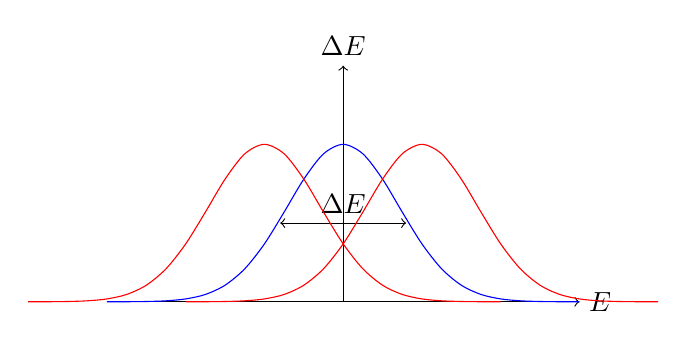
\begin{tikzpicture}
                \draw[->] (-3,0) -- (3,0) node[right] {$E$};
                \draw[->] (0,0) -- (0,3) node[above] {$\Delta E$};
                \draw[domain=-3:3,smooth,variable=\x,blue] plot ({\x},{2*exp(-\x*\x)});
                \draw[<->] (-0.8,1) -- (0.8,1) node[midway,above] {$\Delta E$};

                % draw overlapping gauusian curves displaced by +- 1
                \draw[domain=-3:3,smooth,variable=\x,red] plot ({\x-1},{2*exp(-\x*\x)});
                \draw[domain=-3:3,smooth,variable=\x,red] plot ({\x+1},{2*exp(-\x*\x)});
            \end{tikzpicture}
            \caption{Spektrale Linienbreite. Einzelner Peak in blau, mögliche Überlagerung in rot. Siehe FWHM.}
        \end{figure}
    \end{Antwort}

    \begin{Frage}
        Wie funktioniert ein Laser?
    \end{Frage}
    \begin{Antwort}
        Am Beispiel eines vier Niveau Lasers. 
        \begin{figure}[H]
            \centering
            \includegraphics[width=8cm]{Bilddateien/Lasing.svg.png}
            \caption{Schematische Darstellung eines Vier-Nievau-Lasers am Beispiel stimulierter Emission.}
            \label{fig:Lasing}
        \end{figure}
        Voraussetzung für die Funktionalität ist eine Schnelle Relaxation von $E_P$ und eine kurze Lebensdauer von $E_L$. Die Anregung von $E_0$ muss dabei schneller sein als die Relaxation von $E_L$ zu $E_0$, um eine Besetzungsinversion stationär zu erreichen. Betrachte nun die Prozesse bei $E_M$ als entscheidendes Niveau. 
        \begin{align*}
            \dv{t}N_{E_M}^{(P)}(t) = \eta\cdot W_{1\to 4}\cdot N_{E_1}(t), \tag{P}
        \end{align*}
        wobei $\eta$ die Pumpeffizienz angibt. Dabei nehmen wir die sehr schnelle Entvölkerung von $E_P$ an: $N_{E_P} \approx 0$. 
        \[
            \dv{t}N_{E_M}^{(S)}(t) = -\frac{1}{\tau_S}\cdot N_{E_M}^{(S)}(t). \tag{S}
        \]
        Hierbei ist $\tau_S$ die Lebensdauer von $E_M$, siehe oben. 

        Es kann jedoch ebenfalls zwischen $E_M$ und $E_L$ eine induzierte Absorbtion stattfinden:
        \[
            \dv{t}N_{E_M}^{(I)}(t) \propto p\cdot (N_{E_L}^{(I)}(t) - N_{E_M}^{(I)}(t)). \tag{I}
        \]
        Dabei ist $p$ die Photonendichte des herrschenden Laserfeldes um das Atom herum. Sei $k$ hier die Proportionalitätskonstante, dann gilt im Summation
        \[
            \dv{t}N_{E_M}(t) = \eta\cdot W_{1\to 4}\cdot N_{E_1}(t) - \frac{1}{\tau_S}\cdot N_{E_M}(t) + k\cdot (N_{E_L}(t) - N_{E_M}(t)).
        \]

        Für die Photonendichte erhält man dann 
        \[
            \dv{t}p(t) = p(t)\cdot\nbra{k\cdot n - \frac{1}{\tau_{ph}}}.
        \]

        \subsubsection*{Statische Lösungen}
        Da praktisch jedoch weder Pumprate, noch Photonendichte messbar sind, verlassen wir uns auf die Output-Leistung $P_o$ als Funktion der Inputleistung $P_p$ mit einer Grenze $P_{th}$, ab welcher der Laser zu leuchten beginnt:
        \[
            P_a(P_p) = \alpha_S\cdot (P_p - P_{th}), \tag{P}
        \]
        wobei hier der lineare Zusammenhang relevant ist und $\alpha_S = \eta\cdot E_{3,2}/E_{4,1} \cdot T/(T + L)$ die Steigungseffizienz mit folgenden Parametern ist:
        \begin{itemize}
            \item $\eta$ die Pumpeffizienz,
            \item $T$ die Transmission des Resonators,
            \item $L$ die Verluste des Resonators,
            \item $E_{3,2}$ die Energiedifferenz zwischen $E_3$ und $E_2$ und
            \item $E_{4,1}$ die Energiedifferenz zwischen $E_4$ und $E_1$.
        \end{itemize}
        Der Quotient $E_{3,2}/E_{4,1}$ heißt \emph{quantum efficiency}.
        Als Funktion sieht das ganze dann so aus:
        \begin{figure}[H]
            \centering
            \includegraphics[[width=0.7\textwidth]]{Bilddateien/Pumpleistung.png}
            \caption{Outputleistung als Funktion der Inputleistung.}
            \label{fig:Pumpleistung}
        \end{figure}
        Beim Laserbau muss ebenfalls nach $T$ und $L$ optimiert werden, wodurch sich jedoch die Output Leistung reduziert. 
        \begin{figure}[H]
            \centering
            \includegraphics[width=8cm]{Bilddateien/TOptimierung.png}
            \caption{Optimierung der Outputleistung durch Variation der Transmission $T$.}
        \end{figure} 

        \subsubsection*{Variierende Lösungen}
            Als ersten Kontakt mit nichtstatischen Lösungen betrachten wir das Einschalten der Pumpe. Bis zum Erreichen von $P_{ph}$ gibt es quasi keine angeregten Nd Atome. Ab diesem Punkt wird jedoch ein Photonenfeld $p(t)$ erzeugt, wodurch die Änderungsrate von $p$ groß wird. 

    \end{Antwort}

    \begin{Frage}
        Optische Resonatoren.
    \end{Frage}
    \begin{Antwort}
        Grundätzlich unterscheiden wir zwischen \emph{planparallelen}, \emph{hemispheärischen} und \emph{sphärischen} Resonatoren.
        \begin{figure}[H]
            \centering
            \includegraphics[width=8cm]{Bilddateien/ResonatorBasic.png}
            \caption{Schematische Darstellung eines optischen Resonators \cite{exp8-paper}.}
            \label{fig:OptischerResonator}
        \end{figure}
        Zur Stabilität lassen sich für gegebene Krümmungsradien $R_1$ und $R_2$ die \emph{Gaußschen Resonatorparameter} $g_1$ und $g_2$ definieren:
        \[
            g_1 = 1 - \frac{L}{R_1}, \qquad g_2 = 1 - \frac{L}{R_2}.
        \]
        Die Abbildung zeigt dann das Stabilitätsgebiet mit $g_1\cdot g_2\in [0,1]$.
        \begin{figure}[H]
            \centering
            \includegraphics[width=8cm]{Bilddateien/StabileGebiete.png}
            \caption{Stabilitätsgebiete für optische Resonatoren.}
            \label{fig:StabileGebiete}
        \end{figure}
        In diesem Resonator können sich nun stehende Wellen ausbilden, welche durch die \emph{Resonatormoden} beschrieben werden. Die Moden sind dabei durch die \emph{Resonatorlänge} $L$ und die Lichtwellenlänge $\lambda$ gegeben; Lösungen sind $\lambda_n/2\in\N$ mit 
        \[
            \frac{\lambda_n}{2}= \frac{L}{n}\implies \lambda_{n+1} - \lambda_n = \frac{2L}{n\cdot (n+1)} = \frac{c}{2\cdot L}.  
        \]
        Im Beispiel des NdYAG Lasers können demnach bei $L = 50\si{\mm}$ und $\Delta\lambda = 3\si{\giga\hertz}$ etwa $n = 30$ Moden auftreten mit $\lambda = 1064\si{\nano\meter}$.
    \end{Antwort}

    \begin{Frage}
        Lasertypen.
        \begin{itemize}
            \item Halbleiterlaser (Beispiel AlGaAs)
            \item Festkörperlaser (Beispiel Nd:YAG)
        \end{itemize}
    \end{Frage}
    \begin{Antwort}
        \subsection*{Aluminium-Gallium-Arsenid Laser}
            
        \subsubsection*{Neodym-YAG Laser}
            Der Neodym-YAG Laser ist ein Festkörperlaser, welcher durch Pumpen mit einem Blitzlicht erzeugt wird. Der Laser besteht aus einem YAG-Kristall, welcher mit Neodym dotiert ist. Der Kristall wird durch eine Blitzlampe gepumpt, welche durch einen Kondensator geladen wird. Der Kondensator wird durch einen Spannungsimpuls entladen, wodurch die Blitzlampe kurzzeitig sehr hell aufleuchtet. Die Übergänge kann man in der Grafik erkennen:
            \begin{figure}
                \centering
                \includegraphics[width=8cm]{Bilddateien/NdYAGSpektrum.png}
                \caption{Spektrum des Nd:YAG Lasers \cite{exp8-paper}.}
                \label{fig:NdYAGSpektrum}
            \end{figure}
            Der strahlungsfreie Übergang kann dabei durch Phononen vermittelt werden. Der Neodym Laser stellt dabei einen Vier-Niveau-Laser dar: Da die Nd Atome in dem YAG Kristall eingebettet sind, entsteht das Grundniveau $^4I_{9/2}$ und das Zielniveau $^4F_{3/2}$. Durch Aufspaltung von $^4I_{9/2}$ können vier Übergänge mit leicht variierenden Wellenlängen gepumpt werden. Daraufhin wird durch strahlungslose Übergänge das Niveau $^4F_{3/2}$ besetzt. Durch spontane Emission kann unter drei Lichtfrequenzen die folgenden Niveaus erreicht werden:
            \begin{itemize}
                \item $^4I_{13/2}$ mit Wellenlänge $\lambda = 1322\si{\nano\meter}$
                \item $^4I_{11/2}$ mit Wellenlänge $\lambda = 1064\si{\nano\meter}$
                \item $^4I_{9/2}$ mit Wellenlänge $\lambda = 946\si{\nano\meter}$.
            \end{itemize}
            Durch Relaxion fallen die Nd Atome zurück in den Grundzustand. Das Schema ist optisch das folgende:
            \begin{figure}
                \centering
                \includegraphics[width=8cm]{Bilddateien/SchemaNdYAG.png}
                \caption{Schematische Darstellung des Nd:YAG Lasers \cite{exp8-paper}.}
                \label{fig:SchemaNdYAG}
            \end{figure}
            Die Übergänge können dabei durch Photonenstrahlung oder mechanische Interaktionen wie Kollisionen oder Vibrationen vermittelt werden. 
    \end{Antwort}

    \begin{Frage}
        Diodenlaser.
        \begin{itemize}[label=$\to$]
            \item Wie funktioniert der Pumpmechanismus?
            \item Was versteht man unter Modenselektion?
            \item Was sind die Vor- und Nachteile als Pumplaser?
        \end{itemize}
    \end{Frage}
    \begin{Antwort}


        \begin{table}
            \centering
            \begin{tabular}{|c|c|}\hline
                \textbf{Vorteil} & \textbf{Nachteil} \\\hline\hline
                $50-80\si{\percent}$ Effizienz & max. $10\si{\watt}$ Output\\
                kleine Größe & \\
                gute Kombinierbarkeit & \\

            \end{tabular}
        \end{table}
    \end{Antwort}

    \begin{Frage}
        Wie ist das zeitliche Verhalten eines Lasers (Spiking)?
    \end{Frage}
    \begin{Antwort}
        Bei starken Störungen des Gleichgewichtszustands der Besetzungsinversion $n$ und der Photonendichte treten anharmonische Schwingungen auf. Diese können erwünscht oder unerwünscht sein:\\

        \textbf{Spiking}. Wird der Laser eingeschaltet, wird erstmal keine Photonendichte $p$ vorhanden sein. Erst, wenn die Laserleistung $P_a$ einen Schwellwert $P_{th}$ überschreitet, kann prinzipiell $p>0$ sein. Da sich die Photonen im Resonator aber mit einer endlichen Geschwindigkeit bewegen, kommt es zunächst einer Überpopulation der Besetzungsinversion. Dadurch können aber anschließend mehr Photonen pro Zeiteinheit erzeugt werden (induzierte Emission), was zu einer Unterbevölkerung führt - dieser Prozess wiederholt sich, bis sich $n$ und $p$ eingeschwungen haben.

        \begin{figure}[H]
            \centering
            \includegraphics[width=0.6\textwidth]{Bilddateien/Spiking.jpg}
            \caption{Output-Leistung eines gepulsten Laser: unten ist der ieale Verlauf, oben ein realer mit Spikes am Anfang jedes Pulses.}
        \end{figure}

        Der erste \textit{Spike} einer solchen Schwingen kann die 100- bis 1000-fache Leistung des Equilibriums hervorrufen und zu Schäden am Material führen!\\

        \noindent\textbf{Q-Switching}. Z.B. durch absorbierende Kristalle im Resonator können Photonverluste dort künstlich hochgehalten werden. Dadurch kann die Besetzungsinversion $n_i$ größer werden als normal möglich ($n_{th}$), da $p\approx 0$ gerade wegen der Absorbtion und dadurch keine induzierte Emission stattfinden kann. Wird der Kristall nun entfern, kommt es zu einer Kettenreaktion der Photonentladung und zu einem kontrollierten Spike mit Peak 
        \[
            p_{max} = n_{th}\cdot\ln(n_{th} / n_i) - (n_{th} - n_i).    
        \]
        
    \end{Antwort}

    \begin{Frage}
        Aspekte der nichtlinearen Optik,
        \begin{itemize}[label=$\to$]
            \item Was sind die Grundprinzipien?
            \item Was ist die Frequenzverdopplung?
            \item Was ist eine Phasenanpassung?
        \end{itemize}
    \end{Frage}
    \begin{Antwort}
        \textbf{Anmerkung}: In der linearen Optik werden u.a. zwei Annahmen gemacht: für Licht gilt das Superpositionsprinzip und die Frequenz von Licht liegt keinen Änderungen zugrunde. 

        \begin{itemize}[label=$\to$]
            \item Prozesse werden grob in zwei Kategorien unterteilt:
            \begin{itemize}
                \item[(A)] Resonante Phenomäne: das Licht bewirkt Übergänge in Materie.
                \item[(B)] Nicht-resonante Phenomäne: das Licht ist zu niederenergetisch, um relevante Übergänge zu bewirken.
            \end{itemize}
            In beiden Fällen gibt es trotzdem eine Wechselwirkung von Licht und Materie. Der Photonenhagel auf ein Medium regt Dipolschwingungen der Elektronen. Der Polarisationsvektor ist bei großen $E$-Feldern aber komplex abhängig von deren Auslenkung. Einer erste nichtharmonische Näherung wäre:
            \[
                P = \chi_L\cdot E + \chi_{NL} \cdot E^2\qquad \chi_L,\chi_{NL}\in\R.    
            \]

            \item Quadratische Effekte wie oben für $P$ können zu einer Frequenzverdopplung führen. Dort wird also auch Licht der doppelten Frequenz gestreut. \textit{Allerdings muss $P$ auch anharmonisch sein, also richtungsunabhängig}. Ansonsten lässt sich mittels Zerlegung des erzeugten Lichts in eine Fourierreihe zeigen, dass keine geraden Koeffizienten auftreten können (also keine Frequenzverdopplung, -vervierfachung, ...). Ebenso sollte das Medium eine hohe Suszeptibilität haben. Beides kann man mit Kristallen bestimmter, richtungsunabhängiger Gitterstruktur realisieren.\\
            
            Der Effizienzgrad von Frequenzverdopplung ist gegeben durch 
            \[
                \nu_{SHG} = \frac{P_{2f}}{P_f} \propto P_f\cdot  F(\delta k).    
            \]
            Dabei sind $P_{2f}$, $P_f$ die Leistungen der Wellen mit Frequenz $2f$, $f$; $F$ ist eine Funktion die für das Argument $\delta k=0$ maximal Eins wird; und $\delta k = k_{2f} - k_f$ ist die Differenz der Wellenvektorbeträge der Wellen mit Frequenzt $2f$, $f$. 
        
            \item Maximale Effizienz wird also erreicht durch $k_{2f} - k_f$. Quantenmechanisch haben wir zwei Photonen mit Vektor $k_f$, die absorbiert werden und so ein Photon mit Vektor $k_{2f}$ erzeugt wird. Die Impulserhaltung verlangt also idealerweise $2\cdot k_f = k_{2f}$. Zusammen mit der Dispersionrelation
            \[
                k_{f'} = \frac{2\pi}{n(f')\cdot\lambda_0}    
            \]
            mit $\lambda_0$ als Wellenlänge \textit{im Vakuum}, führt dies auf $n(2f) = n(f)$ (???). Genau dann schwingen beide Wellen in Phase. Um dies zu erfüllen, braucht man nichtisotrope Medien. Man zielt dort auf
            \[
                n_o(f) = n_{ao}(\theta)(2f)    
            \]
            ab, wobei $n_o$ der ordentliche Brechungsindex ist und $n_{ao}(\theta)$ der außerordentliche ist für einen Winkel $\theta$  zur optischen Achse. Folgende Abbilung illustriert dies:
            
            \begin{figure}[H]
                \centering
                \includegraphics[width=0.6\textwidth]{Bilddateien/Phasenanpassung (Doppelbrechender Kristall).jpg}
                \caption{Die gewünschte Phasenanpassung geschieht genau für den Strahl mit dem Winkel $\theta$, wo sich $n_o$ und $n_{ao}$ kreuzen. \textit{Die Wellen mit Frequenz $f$ muss hier die ordentliche Welle sein!}}
            \end{figure}

            Bei erfolgreicher Phasenanpassung gilt $P_{2f}\propto P_f^2$!
        \end{itemize}
    \end{Antwort}

    \begin{Frage}
        Wie funktioniert die Detektion von Licht?
    \end{Frage}
    \begin{Antwort}
        
    \end{Antwort}

\end{document}